%\documentclass{article}
%\usepackage[utf8]{inputenc}

\documentclass[12pt]{article}
\usepackage{graphicx} % This lets you include figures
\usepackage{hyperref} % This lets you make links to web locations
\graphicspath{ {./images/} }

\usepackage[rightcaption]{sidecap}
\usepackage{caption}
\usepackage{subcaption}
\usepackage{hyperref}

\usepackage{float}

\usepackage{imakeidx}

\usepackage{listings}
\usepackage{xcolor}

\definecolor{eclipseStrings}{RGB}{42,0.0,255}
\definecolor{eclipseKeywords}{RGB}{127,0,85}
\colorlet{numb}{magenta!60!black}

\lstdefinelanguage{json}{
	basicstyle=\tiny\ttfamily,
	commentstyle=\color{eclipseStrings}, % style of comment
	stringstyle=\color{eclipseKeywords}, % style of strings
	tabsize=2,
	showstringspaces=false,
	breaklines=true,
	frame=lines,
	string=[s]{"}{"},
	comment=[l]{:\ "},
	morecomment=[l]{:"},
	literate=
	*{0}{{{\color{numb}0}}}{1}
	{1}{{{\color{numb}1}}}{1}
	{2}{{{\color{numb}2}}}{1}
	{3}{{{\color{numb}3}}}{1}
	{4}{{{\color{numb}4}}}{1}
	{5}{{{\color{numb}5}}}{1}
	{6}{{{\color{numb}6}}}{1}
	{7}{{{\color{numb}7}}}{1}
	{8}{{{\color{numb}8}}}{1}
	{9}{{{\color{numb}9}}}{1}
}

\lstdefinestyle{DOS}
{
	basicstyle=\scriptsize\ttfamily
}

\makeindex


\title{Manual}
\author{Beau De Clercq}
\date{July 2019}

\begin{document}
\maketitle{}

\tableofcontents

\clearpage
\newpage

\section{Running \& using the app}
\subsection{Starting the app}
In order to run the app, the user needs to execute the \emph{run.sh} script on Mac/Linux or the \emph{run.bat} script on Windows.

\subsection{Usage}


\newpage

\section{API calls}
\subsection{Provinces}
\begin{lstlisting}[language=json]
{"data":{
	"provinces":[
			{"entiteitcode":"A",
			"entiteitnummer":"1",
			"links":[
				{"rel":"detail","url":"https://api.delijn.be/DLKernOpenData/api/v1/entiteiten/1"},
				{"rel":"haltes","url":"https://api.delijn.be/DLKernOpenData/api/v1/entiteiten/1/haltes"},
				{"rel":"lijnen","url":"https://api.delijn.be/DLKernOpenData/api/v1/entiteiten/1/lijnen"},
				{"rel":"gemeenten","url":"https://api.delijn.be/DLKernOpenData/api/v1/entiteiten/1/gemeenten"}],
			"omschrijving":"Antwerpen"},
			{"entiteitcode":"O",
			"entiteitnummer":"2",
			"links":[
				{"rel":"detail","url":"https://api.delijn.be/DLKernOpenData/api/v1/entiteiten/2"},
				{"rel":"haltes","url":"https://api.delijn.be/DLKernOpenData/api/v1/entiteiten/2/haltes"},
				{"rel":"lijnen","url":"https://api.delijn.be/DLKernOpenData/api/v1/entiteiten/2/lijnen"},
				{"rel":"gemeenten","url":"https://api.delijn.be/DLKernOpenData/api/v1/entiteiten/2/gemeenten"}],
			"omschrijving":"Oost-Vlaanderen"},
			{"entiteitcode":"B",
			"entiteitnummer":"3",
			"links":[
				{"rel":"detail","url":"https://api.delijn.be/DLKernOpenData/api/v1/entiteiten/3"},
				{"rel":"haltes","url":"https://api.delijn.be/DLKernOpenData/api/v1/entiteiten/3/haltes"},
				{"rel":"lijnen","url":"https://api.delijn.be/DLKernOpenData/api/v1/entiteiten/3/lijnen"},
				{"rel":"gemeenten","url":"https://api.delijn.be/DLKernOpenData/api/v1/entiteiten/3/gemeenten"}],
			"omschrijving":"Vlaams-Brabant"},
			{"entiteitcode":"L",
			"entiteitnummer":"4",
			"links":[
				{"rel":"detail","url":"https://api.delijn.be/DLKernOpenData/api/v1/entiteiten/4"},
				{"rel":"haltes","url":"https://api.delijn.be/DLKernOpenData/api/v1/entiteiten/4/haltes"},
				{"rel":"lijnen","url":"https://api.delijn.be/DLKernOpenData/api/v1/entiteiten/4/lijnen"},
				{"rel":"gemeenten","url":"https://api.delijn.be/DLKernOpenData/api/v1/entiteiten/4/gemeenten"}],
			"omschrijving":"Limburg"},
			{"entiteitcode":"W",
			"entiteitnummer":"5",
			"links":[
				{"rel":"detail","url":"https://api.delijn.be/DLKernOpenData/api/v1/entiteiten/5"},
				{"rel":"haltes","url":"https://api.delijn.be/DLKernOpenData/api/v1/entiteiten/5/haltes"},
				{"rel":"lijnen","url":"https://api.delijn.be/DLKernOpenData/api/v1/entiteiten/5/lijnen"},
				{"rel":"gemeenten","url":"https://api.delijn.be/DLKernOpenData/api/v1/entiteiten/5/gemeenten"}],
			"omschrijving":"West-Vlaanderen"}
		]
	},
"status":"success"
}
\end{lstlisting}
API call:
\begin{lstlisting}[style=DOS]
/get_provinces
\end{lstlisting}
Return value: a JSON format response object as shown above.
\newpage

\subsection{Lines}
\begin{lstlisting}[language=json]
{"data":{
	"lines":[
			{"bedieningtype":"NORMAAL","entiteitnummer":"1",
			"lijnGeldigTot":"2019-08-31","lijnGeldigVan":"2019-04-22",
			"lijnnummer":"2","lijnnummerPubliek":"2",
			"links":[{"rel":"detail","url":"https://api.delijn.be/DLKernOpenData/v1/beta/lijnen/1/2"}],
			"omschrijving":"Hoboken - P+R Merksem","publiek":true,"vervoertype":"TRAM"},
			{"bedieningtype":"NORMAAL","entiteitnummer":"1",
			"lijnGeldigTot":"2019-08-31","lijnGeldigVan":"2019-04-22",
			"lijnnummer":"3","lijnnummerPubliek":"3",
			"links":[{"rel":"detail","url":"https://api.delijn.be/DLKernOpenData/v1/beta/lijnen/1/3"}],
			"omschrijving":"P+R Merksem - P+R Melsele","publiek":true,"vervoertype":"TRAM"},
			"{. . .}",
			{"bedieningtype":"NORMAAL","entiteitnummer":"1",
			"lijnGeldigTot":"2019-08-29","lijnGeldigVan":"2019-06-02",
			"lijnnummer":"997","lijnnummerPubliek":"Buu",
			"links":[{"rel":"detail","url":"https://api.delijn.be/DLKernOpenData/v1/beta/lijnen/1/997"}],
			"omschrijving":"Buurtbus Brasschaat","publiek":true,"vervoertype":"BUS"},
			{"bedieningtype":"TECHNISCHE_LIJN","entiteitnummer":"1",
			"lijnGeldigTot":"2019-08-31","lijnGeldigVan":"2019-04-22",
			"lijnnummer":"999","lijnnummerPubliek":"999",
			"links":[{"rel":"detail","url":"https://api.delijn.be/DLKernOpenData/v1/beta/lijnen/1/999"}],
			"omschrijving":"Uit- en inrijdende ritten Antwerpen Tram","publiek":false,"vervoertype":"BUS"}
		]
	},
	"status":"success"
}
\end{lstlisting}
API call:
\begin{lstlisting}[style=DOS]
/get_lines/<province>
\end{lstlisting}
Return value: a JSON format response object as (shortened) shown above. This object describes the available lines for the given province.
\newpage

\subsection{Routes \& passings}
\begin{lstlisting}[language=json]
{"data":{
	"routes":[
			["51.2587202","4.4627988"],["51.2580442","4.4624877"],["51.2560165","4.4605994"],
			. . . ,
			["51.1828995","4.3736422"],["51.1828244","4.373138"],["51.1827684","4.3728861"]
		],
		"stops":[
			{"lati":51.2587626674685,"longi":4.46271548234936,
			"name":"P+R Merksem",
			"temp":17.45,"time":["00:35:00","06:35:00"],"weather":"clear sky"},
			{"lati":51.25366088473669,"longi":4.458164614670439,
			"name":"Ringlaan",
			"temp":17.45,"time":["00:36:00","06:36:00"],"weather":"clear sky"},
			{"lati":51.251262697852084,"longi":4.45592564903742,
			"name":"Rerum Novarum",
			"temp":17.45,"time":["00:37:00","06:37:00"],"weather":"clear sky"},
			{ . . . },
			{"lati":51.18318020637612,"longi":4.383688211677621,
			"name":"Schijfwerper",
			"temp":17.44,"time":["01:06:00","07:06:00"],"weather":"clear sky"},
			{"lati":51.18309990244975,"longi":4.378267845704564,
			"name":"Sportstraat",
			"temp":17.44,"time":["01:08:00","07:08:00"],"weather":"clear sky"},
			{"lati":51.18317216965261,"longi":4.37246136797233,
			"name":"Zwaantjes",
			"temp":17.42,"time":["01:09:00","07:09:00"],"weather":"clear sky"}
		]
	},
"status":"success"
}
\end{lstlisting}
API calls:
\begin{lstlisting}[style=DOS]
/get_timetable/<province>/<line>/to/
/get_timetable/<province>/<line>/from/
\end{lstlisting}
Return value: a JSON format response object as (shortened) shown above. This object describes the stops on the line and provides passing times, weather information and coordinates for the route that will be followed. 

\subsection{Other calls}
API calls:
\begin{lstlisting}[style=DOS]
/timetable/static/img/<name>
/timetable/<province>/<line>/static/img/<name>
\end{lstlisting}
Return value: the image saved in the folder \emph{static/img} as \emph{name}.

\newpage

\section{Site links}

\subsection{/}
\begin{center}
	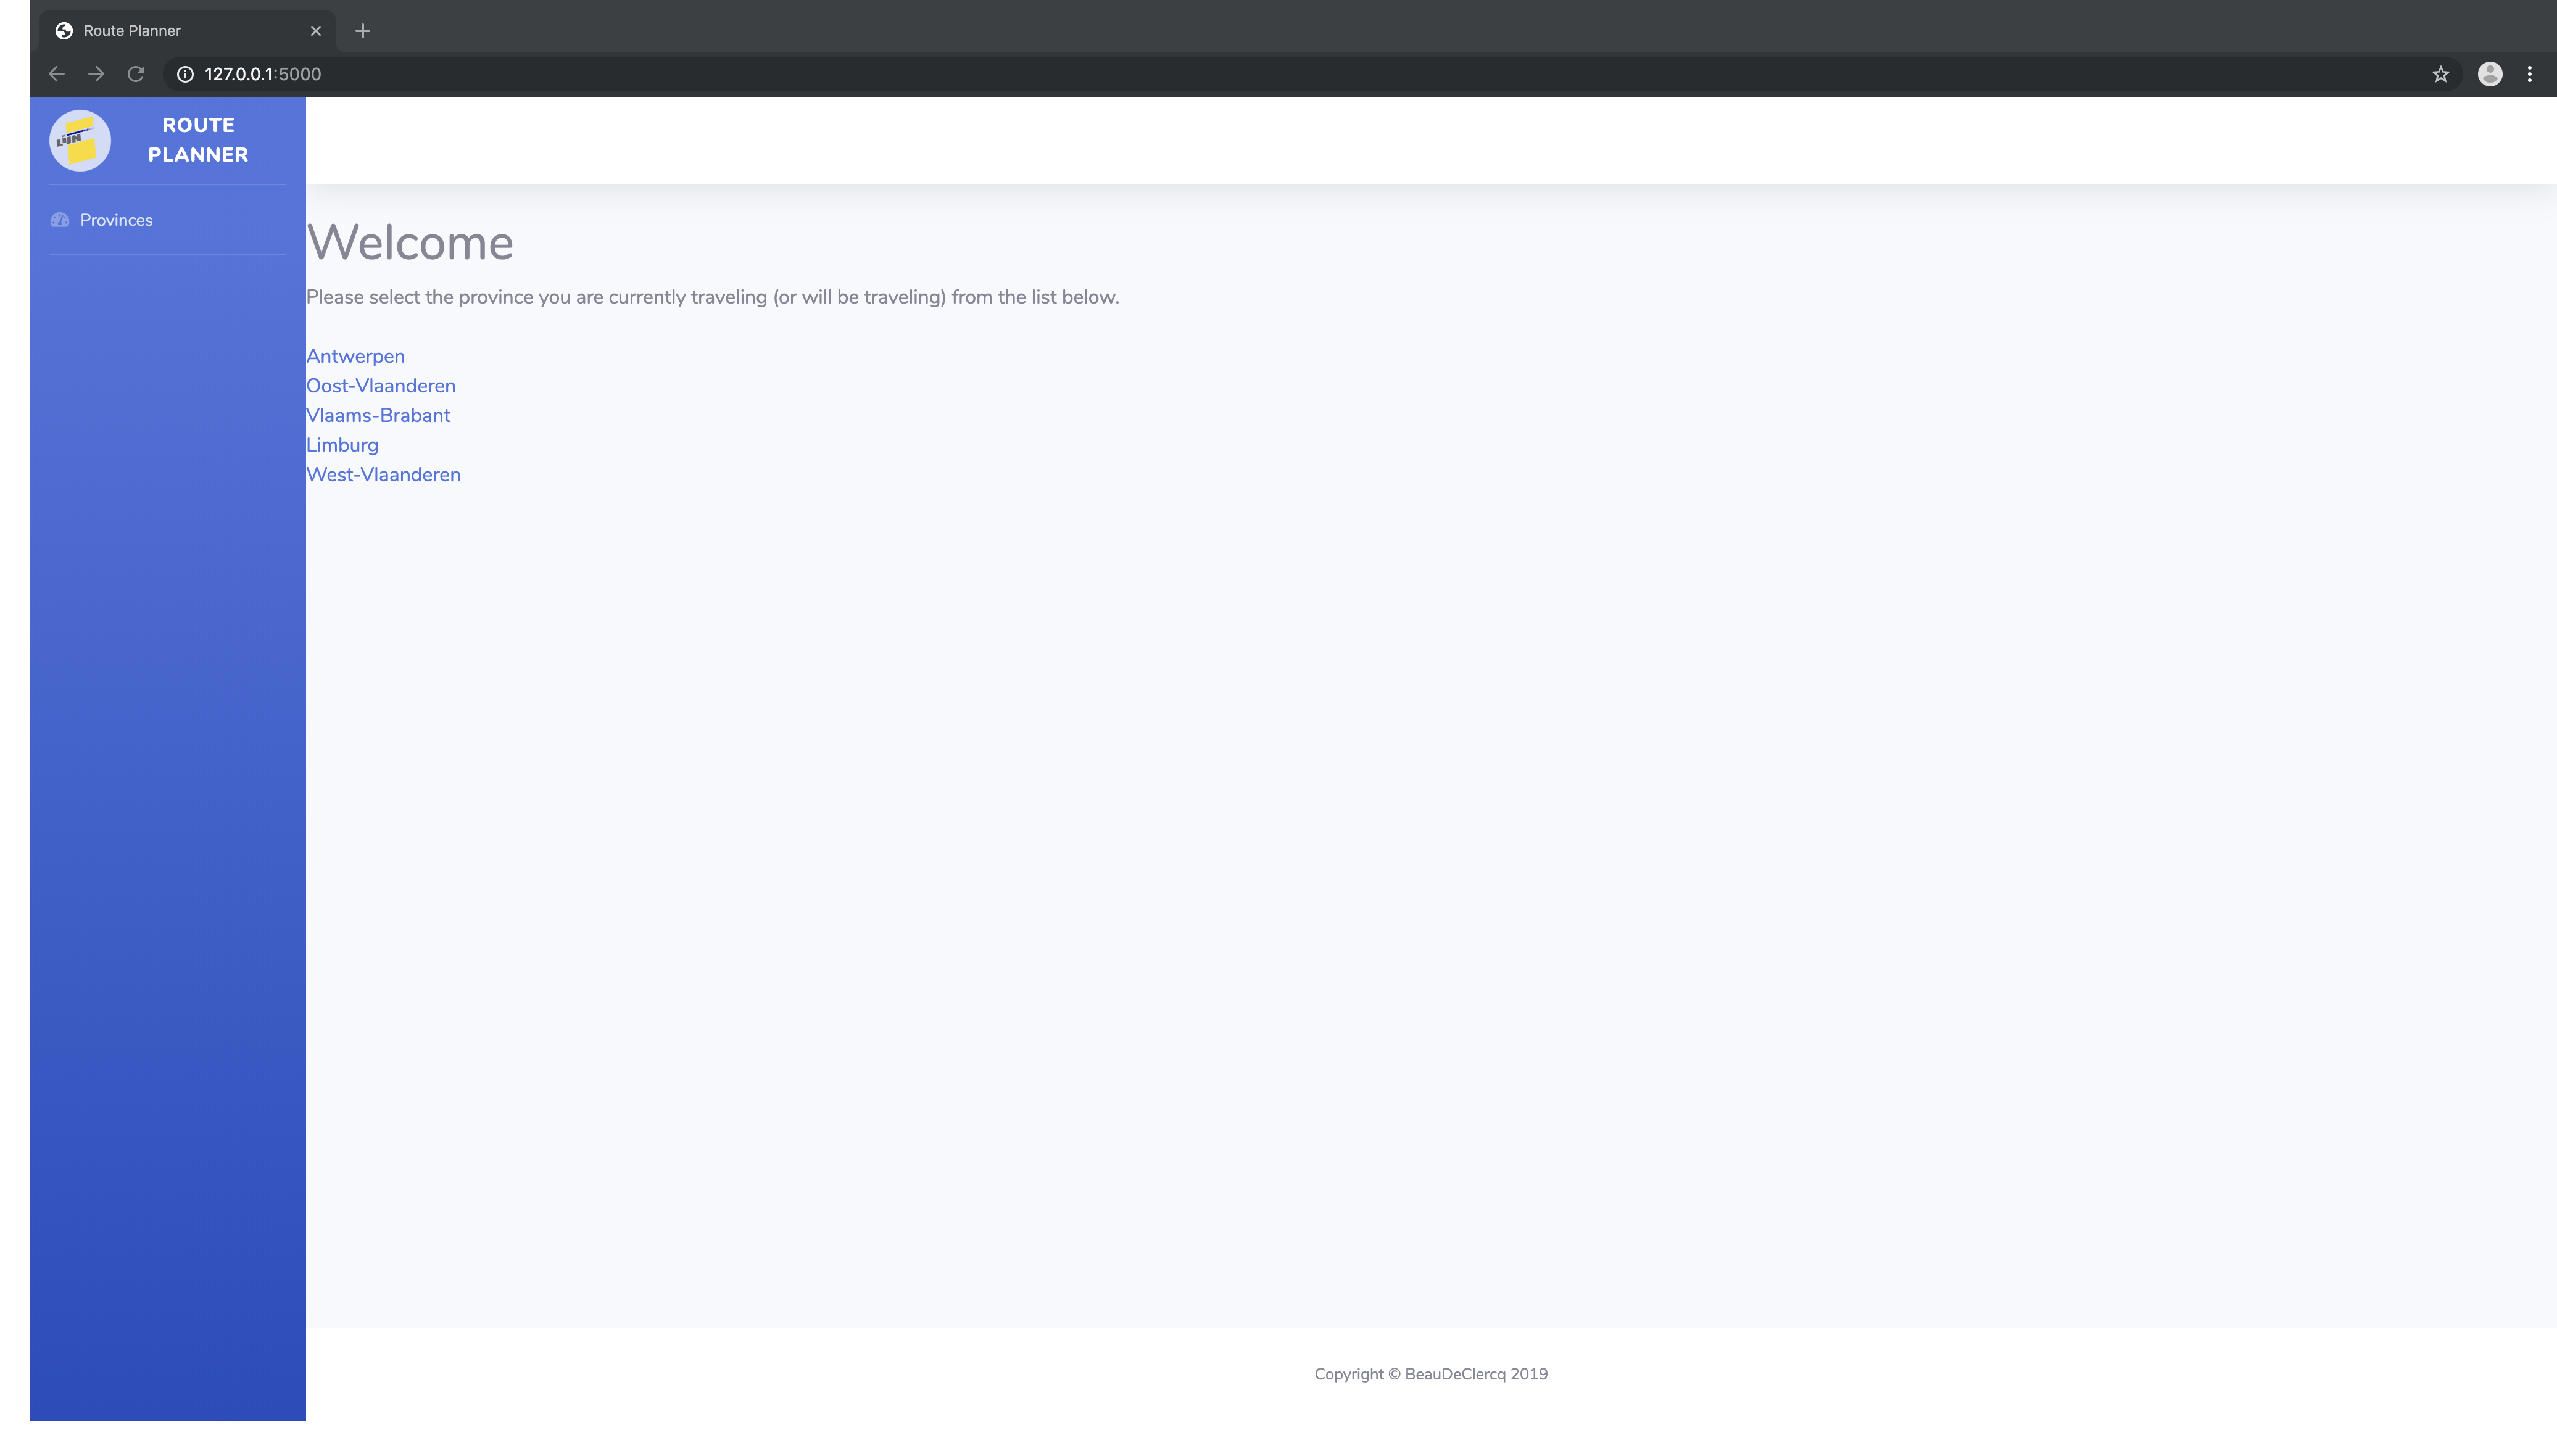
\includegraphics[width=\linewidth]{images/Homepage.png}
	\captionof{figure}{Home page}
\end{center}
At the home page, a user can start the process of planning his/her route by selecting a province.

\subsection{/provinces}
\begin{center}
	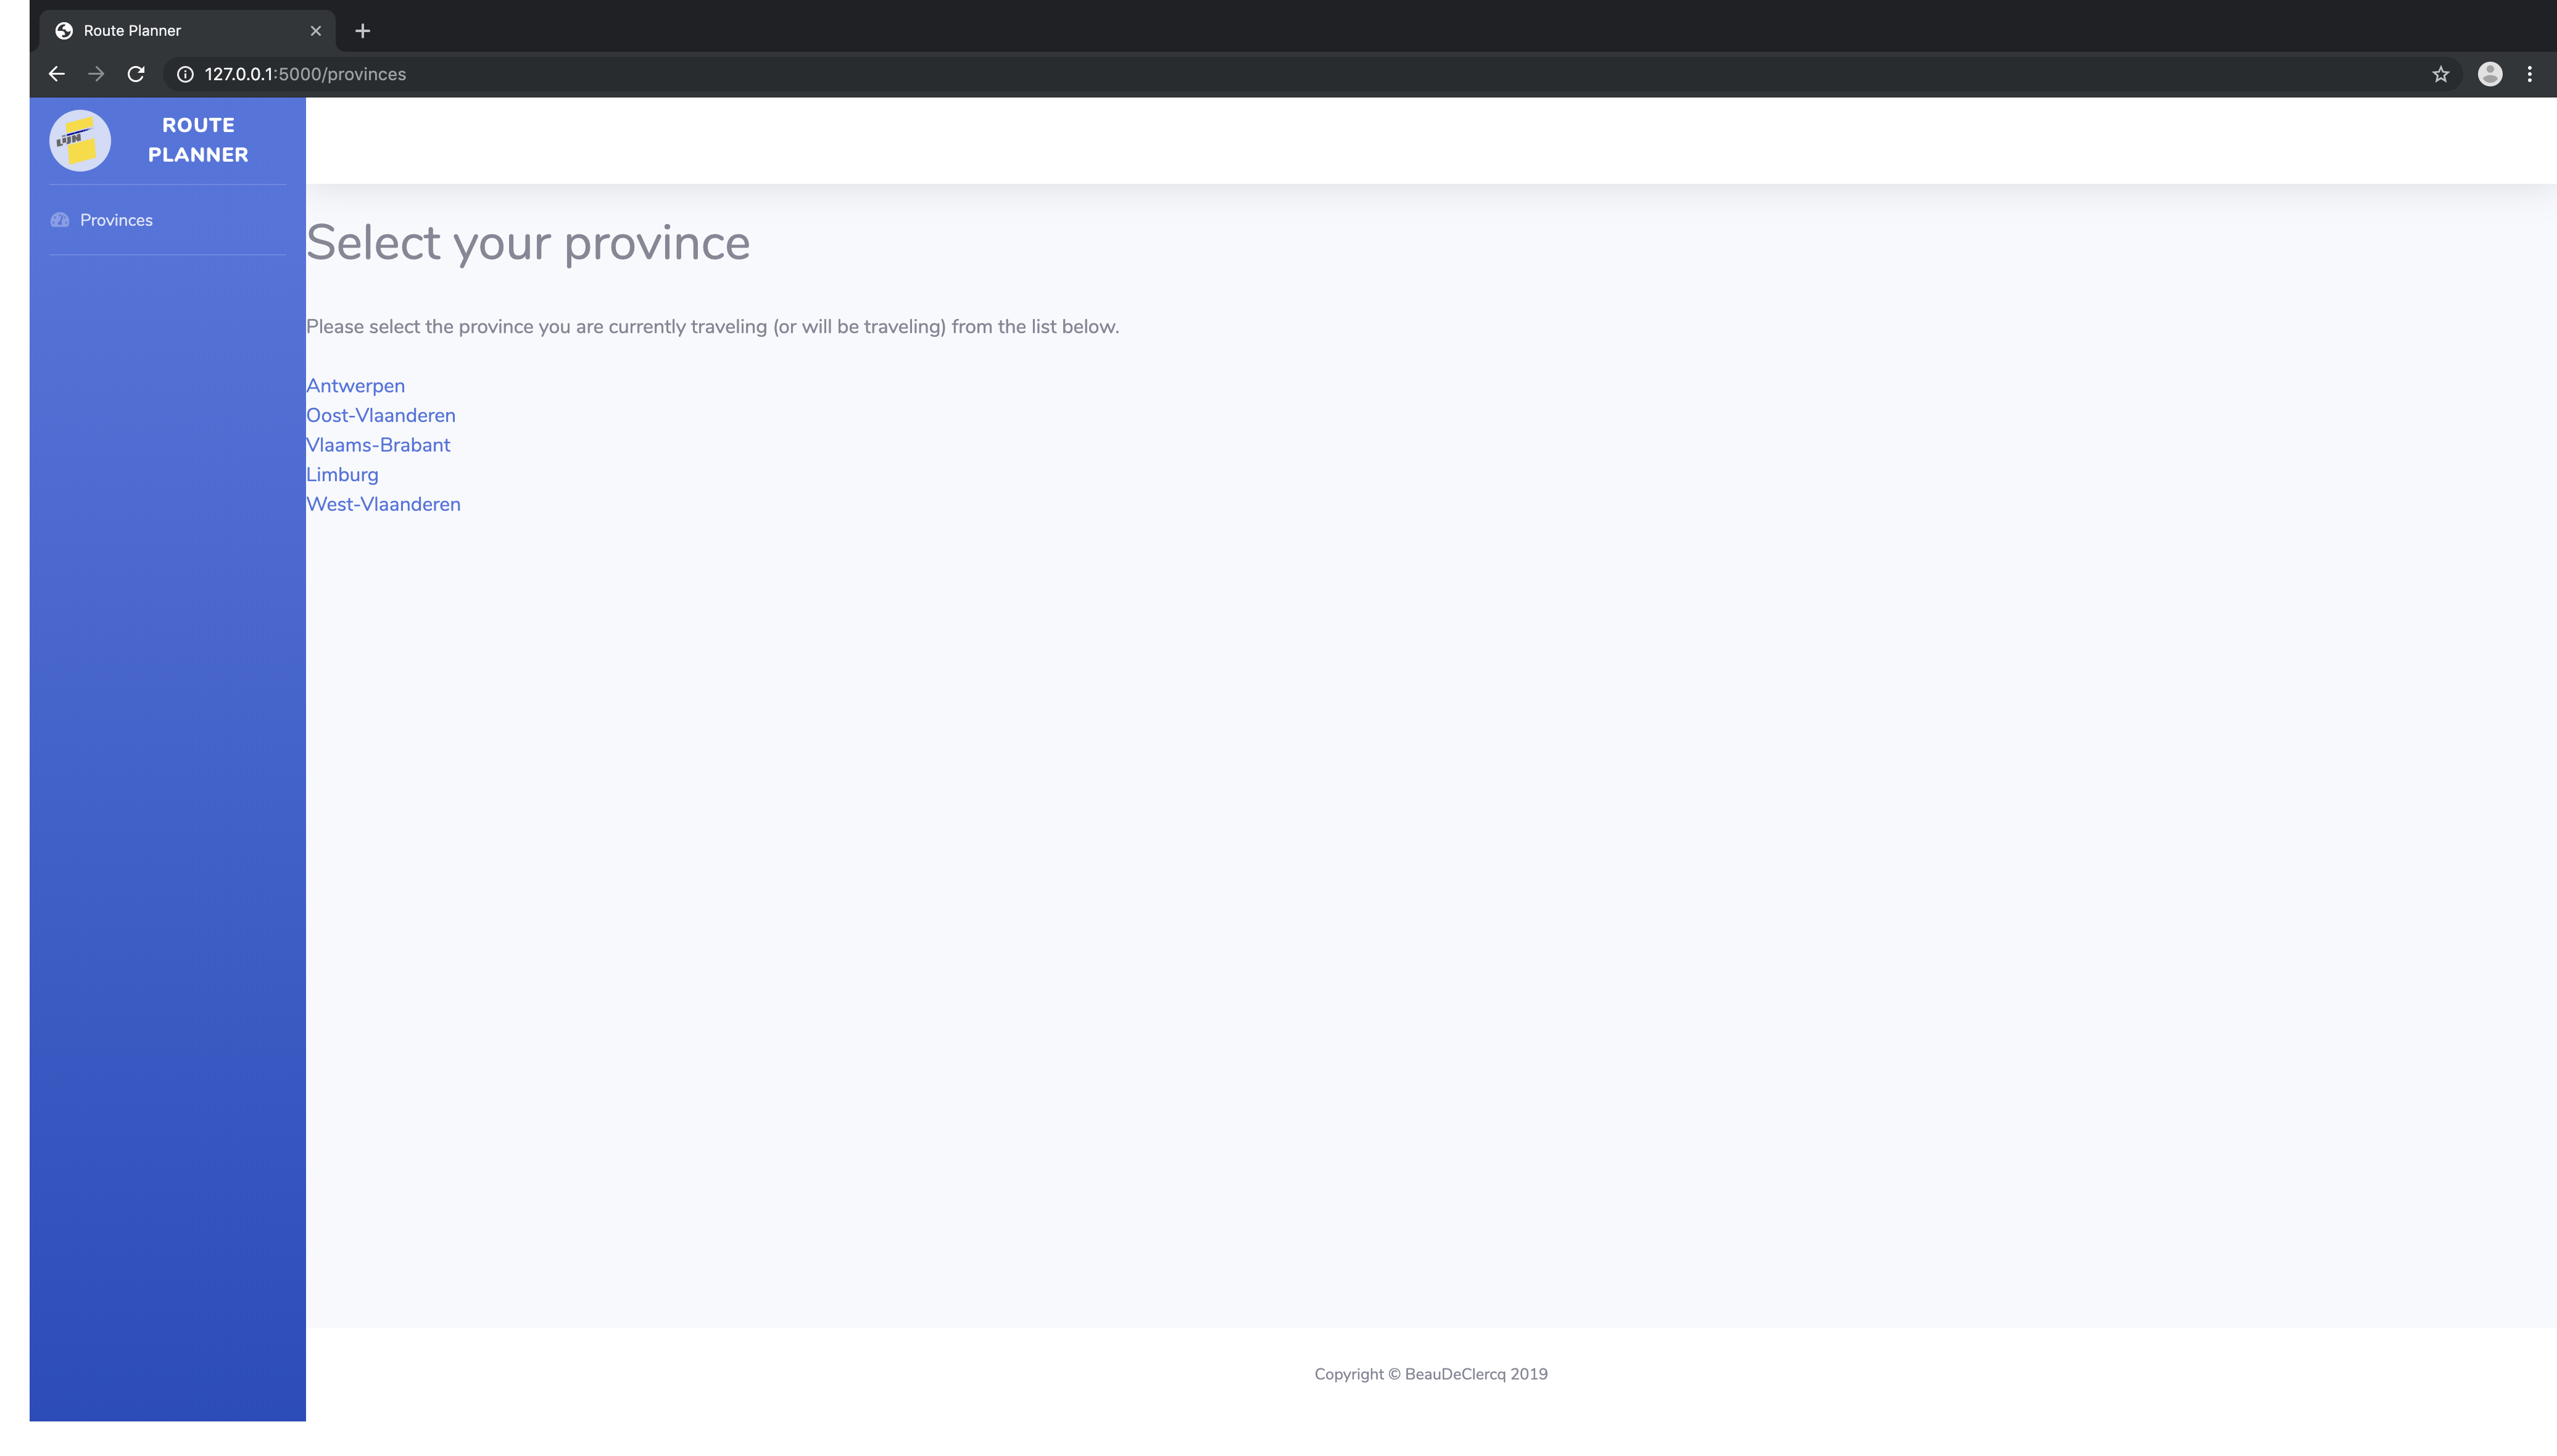
\includegraphics[width=\linewidth]{images/Select_province.png}
	\captionof{figure}{Province page}
\end{center}
At the \lq Provinces page\rq, a user can start the process of planning his/her route by selecting a province. This will take the user to the next step.

\subsection{/lines/$<$province$>$}
\begin{center}
	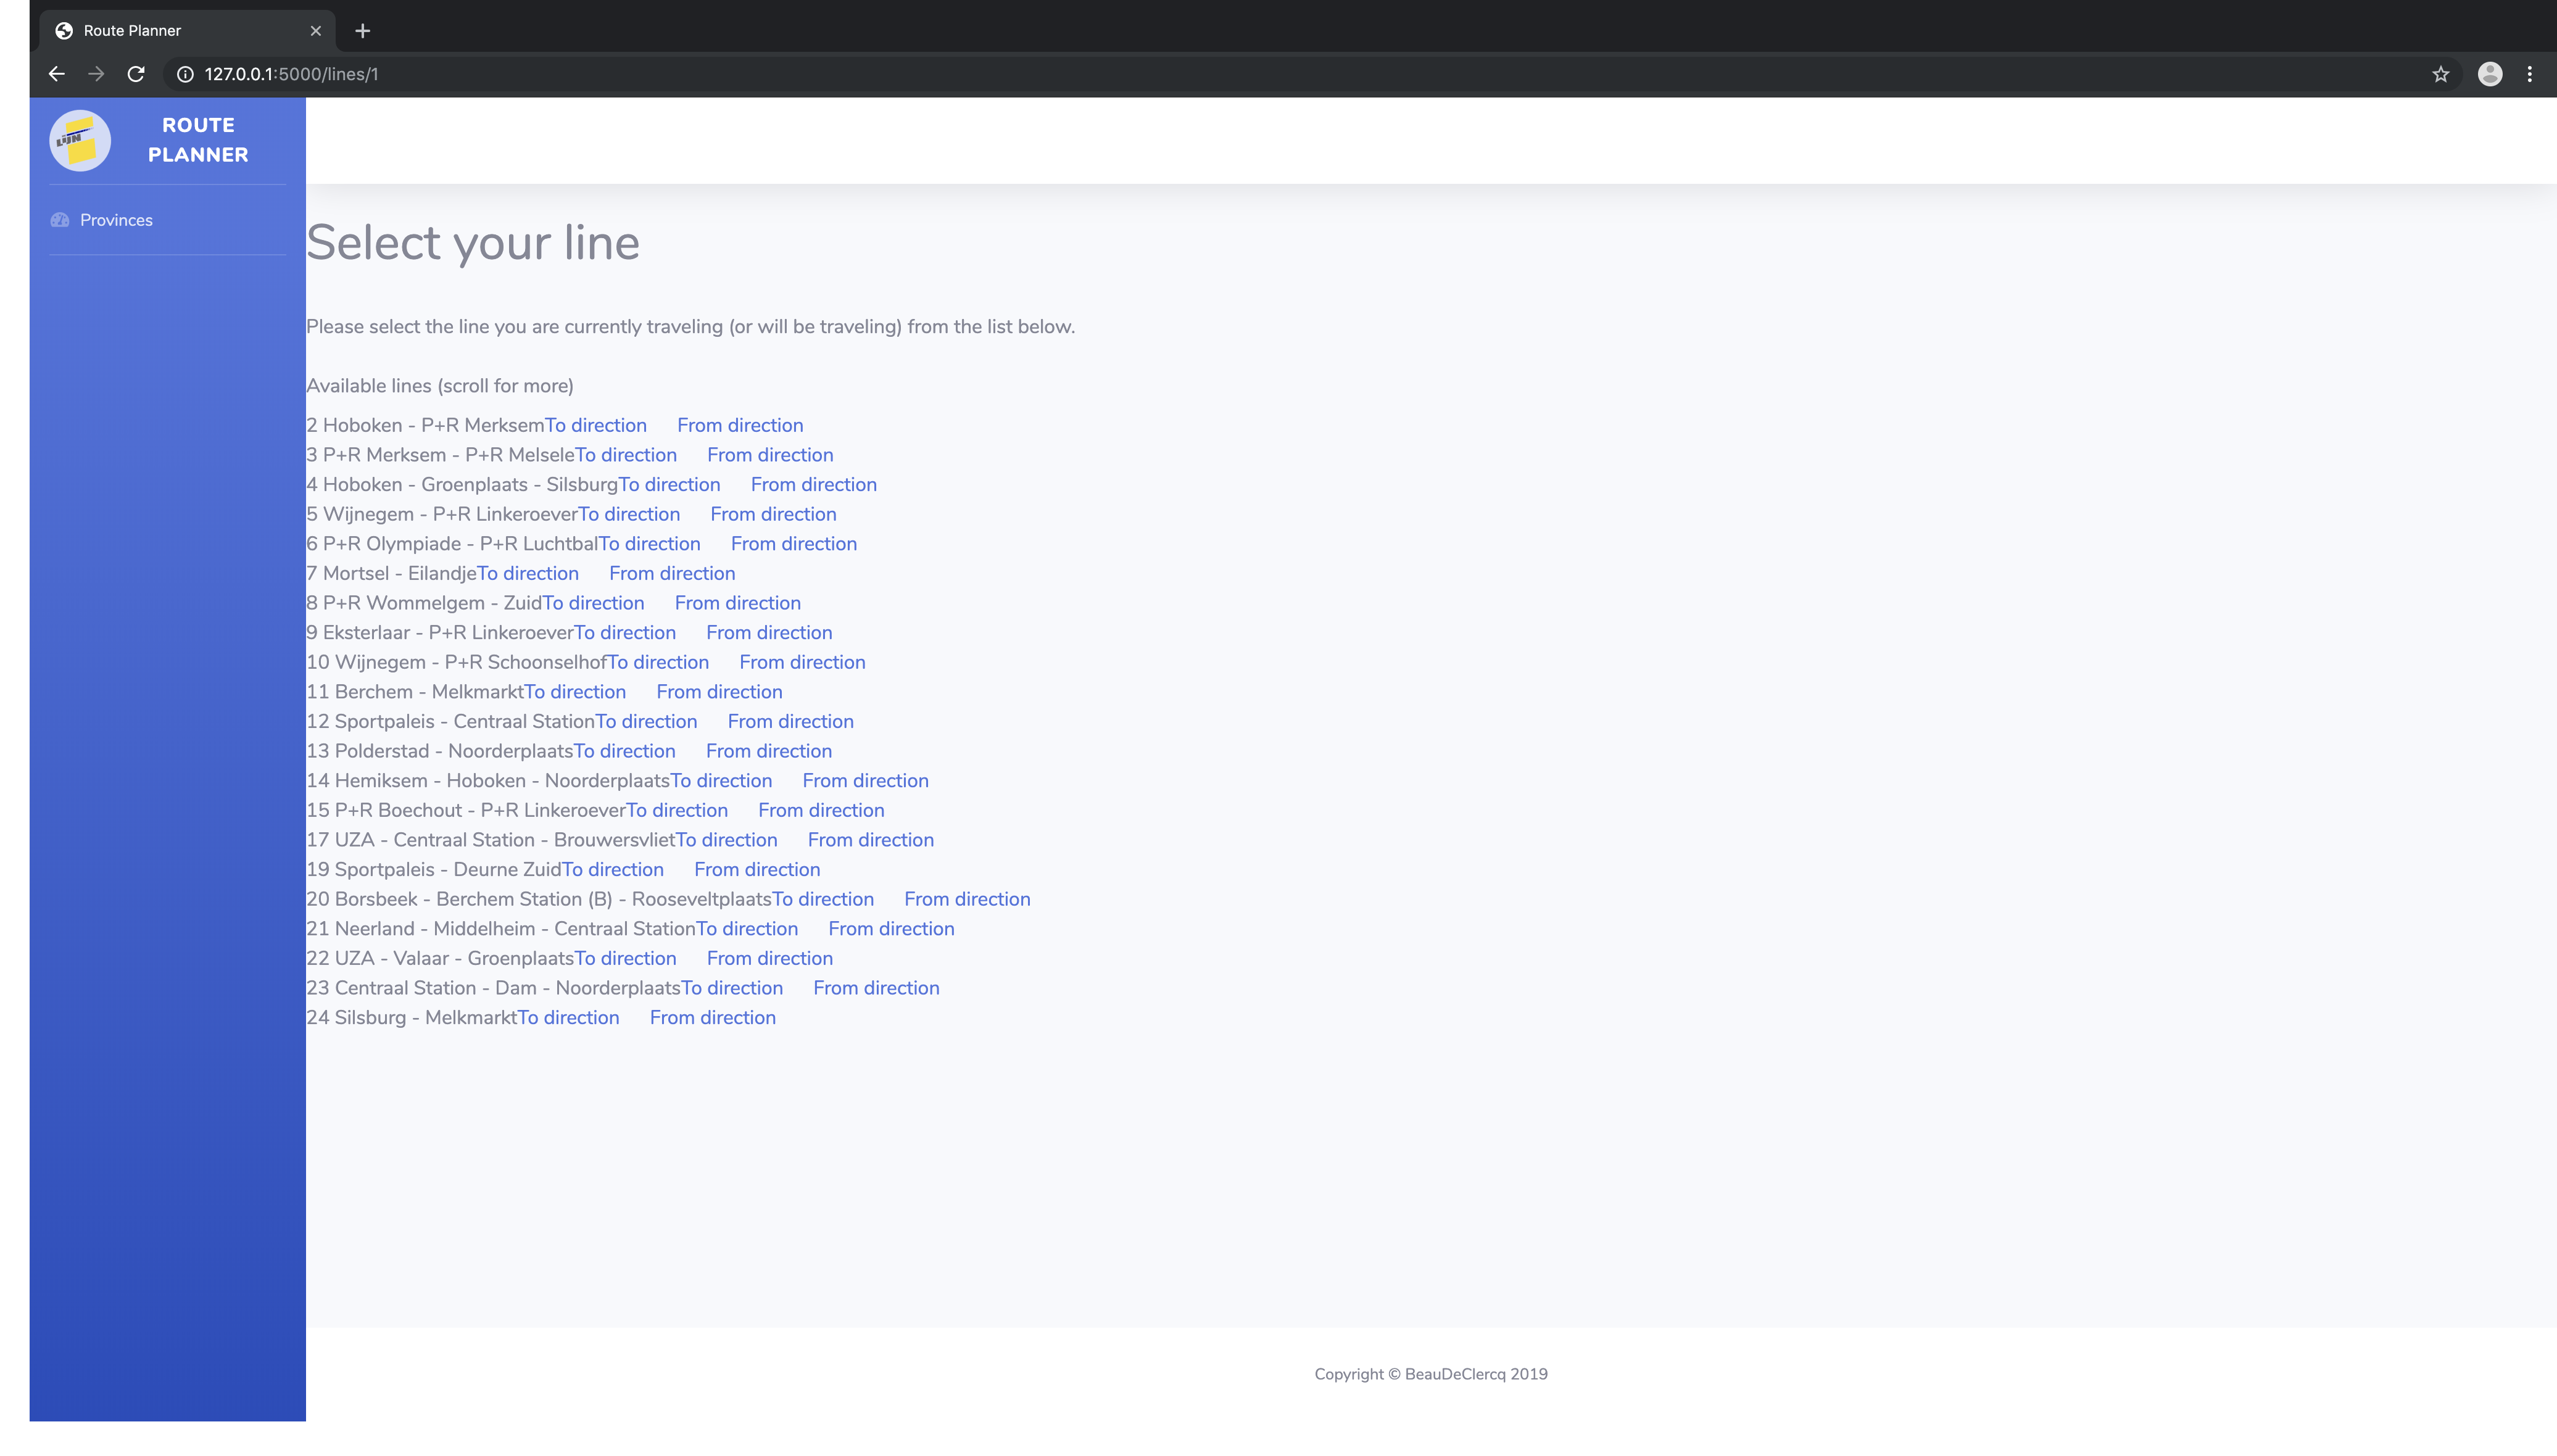
\includegraphics[width=\linewidth]{images/Select_line.png}
	\captionof{figure}{Line selector}
\end{center}
After having selected a province, the user is provided a list of all lines that are available for that province.\\
On the \lq Lines page\rq, the user can then select which direction he or she wants to go.

\subsection{/timetable/$<$province$>$/$<$line$>$/to}
\begin{center}
	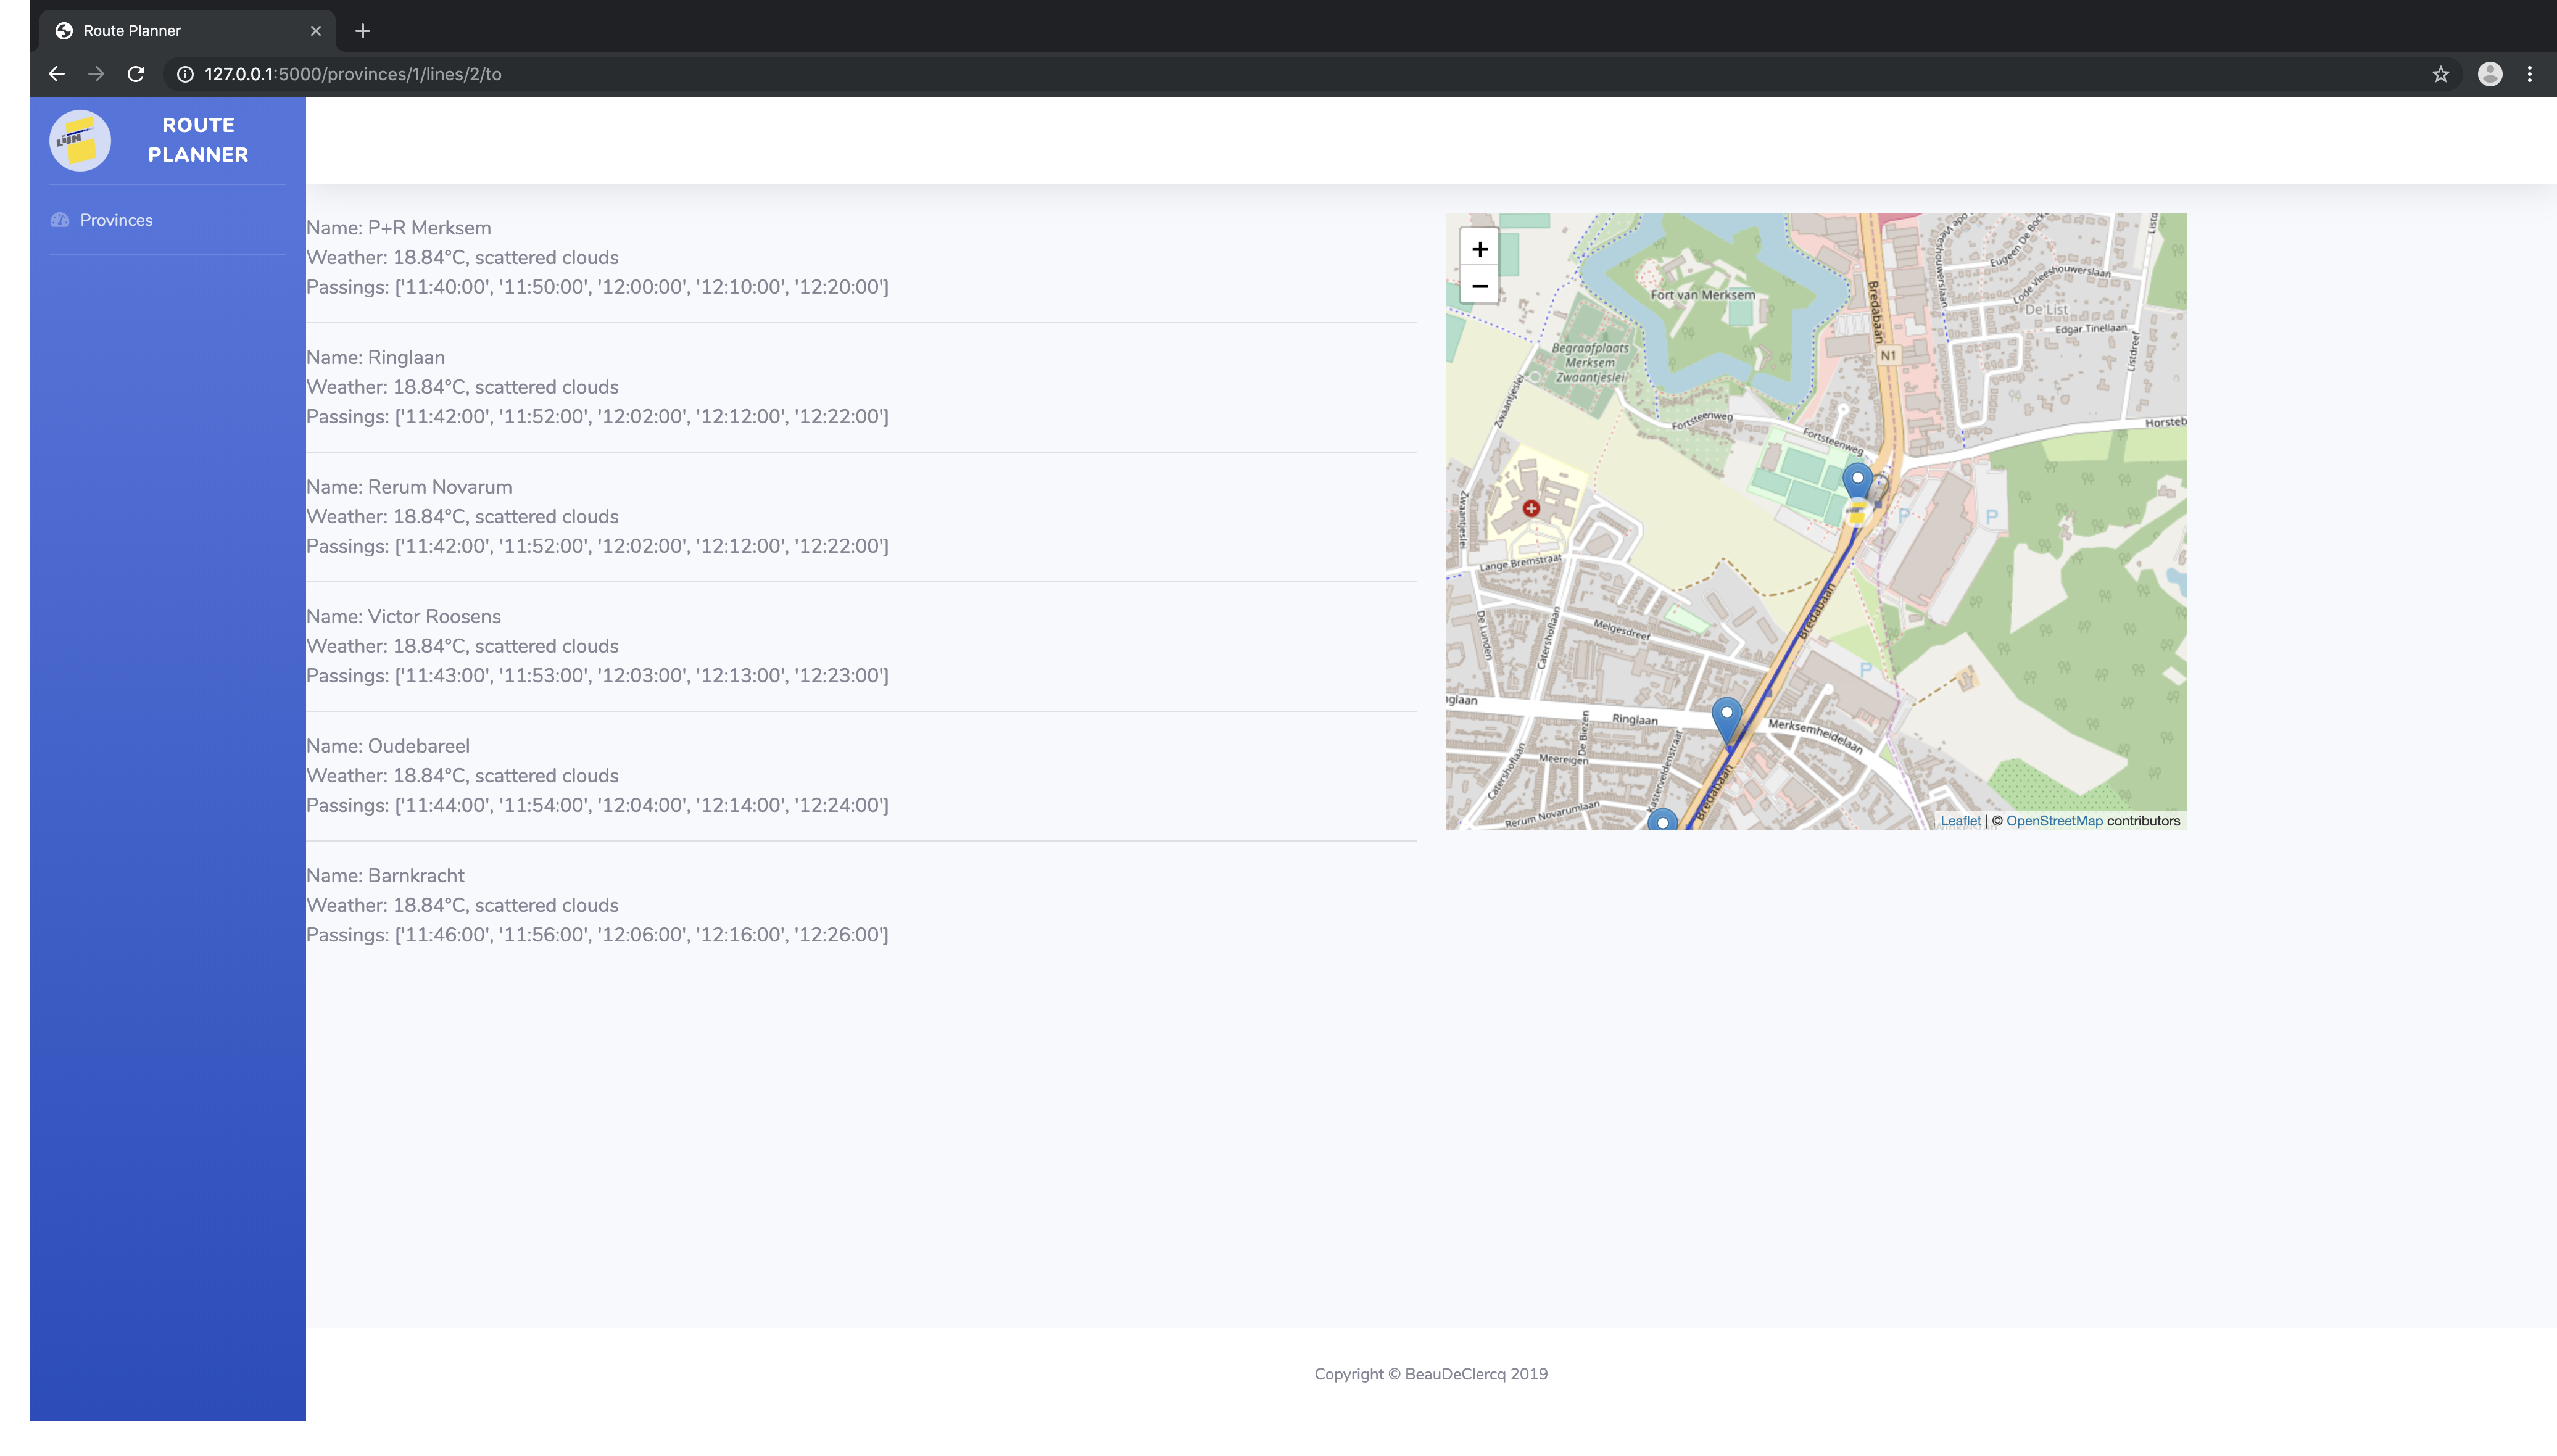
\includegraphics[width=\linewidth]{images/Route_to.png}
	\captionof{figure}{Example route}
\end{center}
Once a direction has been chosen, everything will be processed and  the user will be given a page containing all necessary info.

\subsection{/timetable/$<$province$>$/$<$line$>$/from}
\begin{center}
	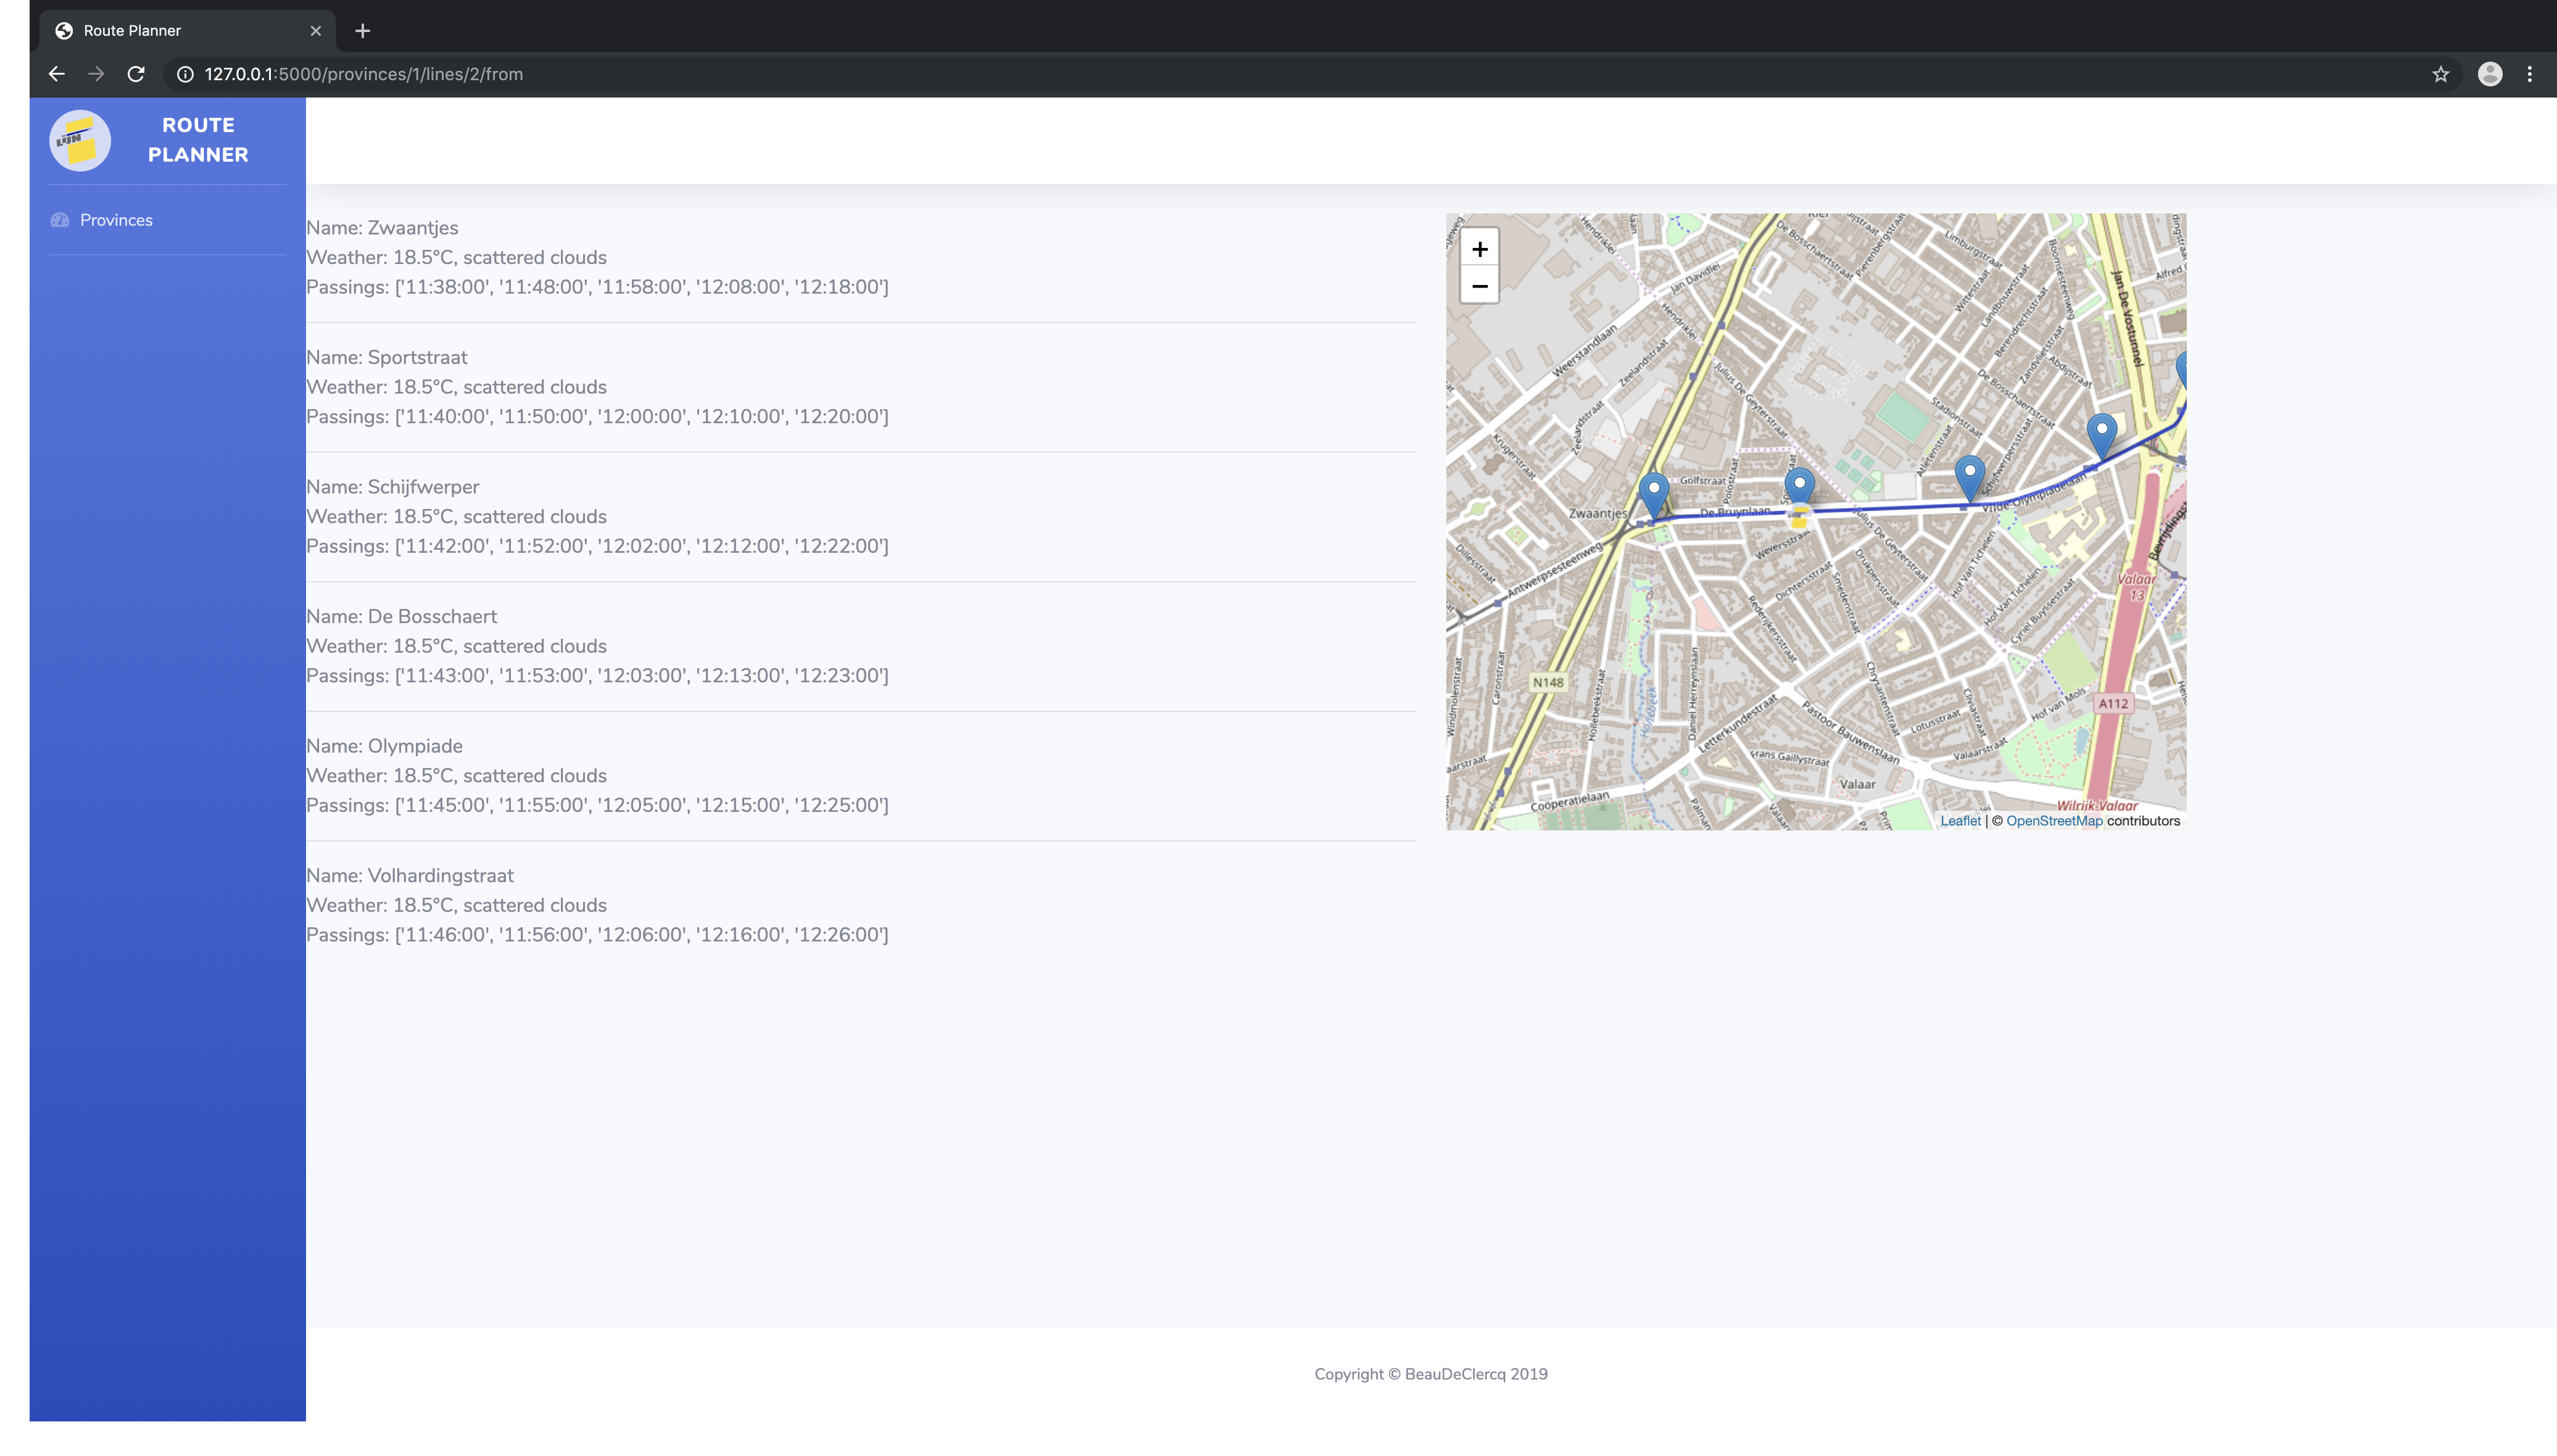
\includegraphics[width=\linewidth]{images/Route_from.png}
	\captionof{figure}{Example route}
\end{center}
Once a direction has been chosen, everything will be processed and  the user will be given a page containing all necessary info.

\newpage

\section{Design choices}


\newpage

\section{Tools used}
\begin{itemize}
	\item Flask as the main framework
	\item Python \emph{requests} module to reduce the lines of code needed to perform an API call
	\item JavaScript \& LeafLet.js for all things map-related

\end{itemize}

\end{document}
